\chapter{User Documentation}
\label{ch:userdoc}

\section{About the Application}

TalkCS is an academic forum platform for universities. It brings question-and-answer
discussions, a course resource library, direct messaging and a shared academic
calendar into a single web application. The software enables students to ask
questions in subject categories, answer and vote on each other's contributions, share
study materials, follow classmates, receive notifications when someone mentions or
answers them, and keep track of exams and deadlines. Teaching staff can moderate
content and publish official calendar events, while administrators manage the
platform as a whole.

\subsection{Target Audience}

TalkCS is intended for the members of a university community:

\begin{itemize}
  \item \textbf{Students}, who need a place to ask course-related questions, find
    answers that were already given, share and download lecture notes and other
    materials, and coordinate with classmates.
  \item \textbf{Professors and teaching assistants}, who want to answer questions in a
    public, reusable way, publish official dates such as exams and assignment
    deadlines, and keep the discussion in their subject organized.
  \item \textbf{Institutional administrators}, who deploy the platform, configure its
    branding and categories, manage user roles, and follow the activity of the
    community.
\end{itemize}

No specialist technical knowledge is required to use TalkCS. Anyone who can use a
modern web browser can register and start participating immediately. Writing posts
supports Markdown, but a toolbar makes the most common formatting available with a
single click, so knowing Markdown is not required.

\subsection{User Roles}
\label{sec:roles}

Every account has exactly one role, which determines what the user is allowed to do.
Newly registered accounts always receive the \emph{Student} role; other roles are
assigned by an administrator (see Section~\ref{sec:guide-admin}).

\begin{table}[H]
  \centering
  \small
  \begin{tabularx}{\textwidth}{@{}l X@{}}
    \toprule
    \textbf{Role} & \textbf{Permissions} \\
    \midrule
    Student & Read and write posts and comments; vote; upload resources; bookmark;
      follow users; chat; create private calendar events and propose public ones;
      edit and delete own content. \\
    Professor & Everything a Student can do, plus: create and edit categories; publish
      public calendar events directly; review (approve or reject) event proposals;
      edit or delete any calendar event; delete any resource. Professors are marked
      with a dedicated badge next to their name. \\
    Admin & Everything a Professor can do, plus: access the Admin Panel (analytics,
      user and role management, branding); archive and restore categories; delete any
      post or comment. \\
    \bottomrule
  \end{tabularx}
  \caption{User roles and their permissions}
  \label{tab:roles}
\end{table}

% =====================================================================
\section{System Requirements}

\subsection{End-User Requirements}

TalkCS is a web application. End users do not need to install any software on their
device. The only requirements are:

\begin{itemize}
  \item A modern web browser: Google Chrome 120 or later, Mozilla Firefox 121 or later,
    Microsoft Edge 120 or later, or Safari 17 or later. JavaScript must be enabled.
  \item A stable internet connection. Real-time features (live comments and chat) use a
    WebSocket connection, which must not be blocked by a firewall or proxy.
  \item A valid e-mail address for registration and for password recovery.
\end{itemize}

The user interface is responsive and can be used on desktop computers, tablets and
mobile phones (from a screen width of about 360 pixels).

\subsection{Developer / Self-Hosting Requirements}

Developers who wish to run the application locally, or institutions that want to host
their own instance, need the following environment:

\begin{table}[H]
  \centering
  \small
  \begin{tabularx}{\textwidth}{@{}l X@{}}
    \toprule
    \textbf{Requirement} & \textbf{Minimum Version / Details} \\
    \midrule
    Operating System & Windows 10/11, macOS 12+, or Linux \\
    Java Development Kit & JDK 21 (the Gradle toolchain is configured for Java 21) \\
    PostgreSQL & 16 or later \\
    Node.js & 20.19 or later (required by Vite 7); npm 10 or later \\
    Git & Any recent stable version \\
    Resend account & Optional; needed only for sending e-mails (free tier is sufficient)~\cite{resend} \\
    Memory & At least 2 GB of free RAM (the backend runs with a 512 MB heap) \\
    \bottomrule
  \end{tabularx}
  \caption{Developer system requirements}
  \label{tab:dev-req}
\end{table}

Gradle itself does not need to be installed, because the repository contains the
Gradle Wrapper (\code{gradlew}), which downloads the correct Gradle version
automatically. The application was developed and tested on the following system:

\begin{itemize}
  \item Operating System: macOS
  \item Java: OpenJDK 21
  \item PostgreSQL: 16
  \item Node.js: 20.x LTS with npm 10.x
  \item Browsers: Google Chrome and Safari
\end{itemize}

% =====================================================================
\section{Installation and Setup}
\label{sec:install}

This section describes how to set up and run TalkCS locally from the source code.

\subsection{Prerequisites}

Install the following tools before proceeding:

\begin{itemize}
  \item Java 21 (for example Eclipse Temurin): \url{https://adoptium.net/}
  \item PostgreSQL 16: \url{https://www.postgresql.org/download/}
  \item Node.js (includes npm): \url{https://nodejs.org/}
  \item Git: \url{https://git-scm.com/downloads}
\end{itemize}

After installation, verify that the tools are available by running these commands in
a terminal:

\begin{lstlisting}[language=bash,caption={Verifying the installed tools},label={lst:verify}]
java -version
psql --version
node --version
npm --version
\end{lstlisting}

To enable e-mail sending (password reset links, mention and accepted-answer
notifications, and the daily digest), create a free account at
\url{https://resend.com/} and generate an API key. Without a key the application
works normally, but e-mails are not delivered.

\subsection{Project Setup}

Clone the repository and install the frontend dependencies:

\begin{lstlisting}[language=bash,caption={Cloning the repository and installing dependencies},label={lst:clone}]
git clone https://github.com/NeonWest/TalkCS.git
cd TalkCS
cd frontend
npm install
cd ..
\end{lstlisting}

The \code{npm install} command downloads all packages defined in
\code{frontend/package.json}, including React, React Router, TanStack Query, the
Markdown editor and the STOMP client. The backend dependencies (Spring Boot, the
PostgreSQL driver, JJWT, etc.) are downloaded automatically by Gradle the first time
the backend is built.

\subsection{Database Setup}

Create an empty PostgreSQL database called \code{talkcs}:

\begin{lstlisting}[language=bash,caption={Creating the database},label={lst:createdb}]
psql -U postgres -c "CREATE DATABASE talkcs;"
\end{lstlisting}

No SQL scripts have to be executed manually. When the backend starts, Hibernate
creates and updates all tables automatically from the entity classes
(\code{spring.jpa.hibernate.ddl-auto=update}), and the twelve milestone badges are
inserted on the first start-up.

\subsection{Environment Configuration}

Create a file named \code{.env} in the root directory of the project and populate it
with the following variables, substituting your own values:

\begin{lstlisting}[language=Properties,caption={Content of \texttt{.env}},label={lst:env}]
DB_USERNAME=postgres
DB_PASSWORD=your-database-password
JWT_SECRET=a-long-random-base64-encoded-secret
RESEND_API_KEY=your-resend-api-key
\end{lstlisting}

The \code{JWT\_SECRET} is used to sign authentication tokens with the HMAC-SHA
algorithm. It must be a Base64-encoded value of at least 32 bytes; a suitable secret
can be generated with \code{openssl rand -base64 64}.

The backend reads further optional variables, listed in Table~\ref{tab:env}. Their
defaults are suitable for local development.

\begin{table}[H]
  \centering
  \small
  \begin{tabularx}{\textwidth}{@{}l X p{0.33\textwidth}@{}}
    \toprule
    \textbf{Variable} & \textbf{Purpose} & \textbf{Default} \\
    \midrule
    \code{SPRING\_DATASOURCE\_URL} & JDBC URL of the database & \url{jdbc:postgresql://localhost:5432/talkcs} \\
    \code{DB\_USERNAME} & Database user & \code{postgres} \\
    \code{DB\_PASSWORD} & Database password & (empty) \\
    \code{JWT\_SECRET} & Base64 key for signing JWTs & development placeholder \\
    \code{RESEND\_API\_KEY} & API key of the e-mail service & \code{dummy} \\
    \code{APP\_BASE\_URL} & Public URL of the frontend (e-mail links, allowed CORS and WebSocket origin) & \url{http://localhost:5173} \\
    \code{PORT} & HTTP port of the backend & \code{8080} \\
    \code{VITE\_API\_URL} & (frontend) URL of the backend API & \url{http://localhost:8080} \\
    \bottomrule
  \end{tabularx}
  \caption{Environment variables}
  \label{tab:env}
\end{table}

\noindent\textbf{Important:} never commit the \code{.env} file to a public repository,
as it contains secret keys. It is excluded from version control via \code{.gitignore}.

\subsection{Starting the Application}

On macOS and Linux, both the backend and the frontend can be started with a single
script from the project root. The script loads the variables from \code{.env}, stops
any process that is still listening on ports 8080 and 5173, and starts both servers:

\begin{lstlisting}[language=bash,caption={Starting backend and frontend together},label={lst:start}]
./start.sh
\end{lstlisting}

Alternatively, the two parts can be started separately in two terminals. This is also
the way to run the application on Windows (using \code{gradlew.bat}):

\begin{lstlisting}[language=bash,caption={Starting the backend and frontend separately},label={lst:start-sep}]
# Terminal 1 - backend (http://localhost:8080)
set -a && source .env && set +a
cd backend
./gradlew bootRun

# Terminal 2 - frontend (http://localhost:5173)
cd frontend
npm run dev
\end{lstlisting}

The application is then available at \url{http://localhost:5173} in the browser.

\subsection{Creating the First Administrator}

For security reasons, the registration form always creates accounts with the Student
role, and only an administrator can change roles. To bootstrap a new installation,
register a normal account through the web interface and then promote it once directly
in the database:

\begin{lstlisting}[language=SQL,caption={Promoting the first administrator},label={lst:first-admin}]
UPDATE users SET role = 'ADMIN' WHERE email = 'admin@university.edu';
\end{lstlisting}

After logging out and back in, the account has access to the Admin Panel, from where
all further role changes can be made through the user interface.

\subsection{Building for Production}

The backend is packaged as a single executable JAR file, and the frontend is compiled
into static files that any web server or static hosting service can serve:

\begin{lstlisting}[language=bash,caption={Building and running for production},label={lst:prod}]
# Backend: produces backend/build/libs/backend-0.0.1-SNAPSHOT.jar
cd backend
./gradlew bootJar
java -jar build/libs/*.jar

# Frontend: produces the static site in frontend/dist
cd frontend
VITE_API_URL=https://api.your-university.edu npm run build
\end{lstlisting}

The repository already contains deployment descriptors for two common hosting
options: \code{backend/nixpacks.toml} describes the build and start commands for
Nixpacks-based platforms~\cite{nixpacks}, and \code{frontend/vercel.json} configures Vercel~\cite{vercel}
to route every path to \code{index.html}, which is necessary for client-side routing.

% =====================================================================
\section{Features Overview}

Table~\ref{tab:features} summarizes all major features of TalkCS.

\begin{longtable}{@{}p{0.27\textwidth} >{\raggedright\arraybackslash}p{0.68\textwidth}@{}}
  \toprule
  \textbf{Feature} & \textbf{Description} \\
  \midrule
  \endfirsthead
  \toprule
  \textbf{Feature} & \textbf{Description} \\
  \midrule
  \endhead
  \bottomrule
  \endfoot
  \bottomrule
  \caption{TalkCS feature overview}
  \label{tab:features}
  \endlastfoot
  Authentication & Registration and login with e-mail and password, JWT-based
    sessions valid for 24 hours, and password recovery via e-mailed one-time links. \\
  Categories & Subject areas (e.g. courses) that group posts, resources and calendar
    events. Created by professors and administrators; can be archived and restored. \\
  Posts & Questions and discussions with Markdown formatting, code syntax highlighting,
    up to five tags and a status (Open, Solved, Closed). \\
  Tag suggestions & Automatic tag proposals based on the title and body of a post. \\
  Similar post detection & Live warning about existing posts that are similar to the
    one being written, to prevent duplicate questions. \\
  Threaded comments & Nested replies of unlimited depth with live updates for all
    readers of the post. \\
  Accepted answers & The question author can accept one answer, which marks the post as
    Solved and rewards the answerer. \\
  Voting and reputation & Up- and down-votes on posts, comments and resources that
    change the author's overall and per-category reputation. \\
  Levels, badges, leaderboard & Five user levels, twelve milestone badges, subject
    expertise badges, and a top-20 leaderboard. \\
  Resource library & Per-category upload, download and voting of course materials (up to
    50 MB per file); trending resources on the home page. \\
  Search & Global search across posts, categories and users. \\
  Trending & The most active posts of the last seven days on the home page. \\
  Profiles and following & Public profiles with bio, avatar, statistics, posts,
    bookmarks and badges; follow and unfollow other users. \\
  Mentions and notifications & \code{@username} mentions, notifications for replies,
    accepted answers and new followers, and a notification bell with unread counter. \\
  E-mail notifications & Immediate e-mails for mentions and accepted answers and a daily
    digest of unread notifications on weekdays. \\
  Direct messaging & Real-time one-to-one chat with unread message counters. \\
  Academic calendar & Month view of exams, deadlines, lectures and other events;
    private events and a public event proposal and review workflow. \\
  Admin Panel & Analytics, user and role management, category management and branding
    configuration. \\
  Theme and layout & Dark and light themes and a responsive layout for mobile devices. \\
\end{longtable}

% =====================================================================
\section{Application User Guide}

This section provides step-by-step instructions for using each feature of TalkCS. It
walks through the functionality from the perspective of a new user, starting with
registration and continuing through each module. Screenshots illustrate the interface
and the key interactions.

\subsection{Authentication}

\subsubsection*{Registration}

To create a new account, open the application and click the link to the registration
page, or navigate directly to \route{/register}. Fill in the form with:

\begin{itemize}
  \item a \textbf{username}, which is displayed next to all your contributions and is
    used for mentions (it must be unique);
  \item a valid \textbf{e-mail address}, which is used for logging in and for
    notifications (it must be unique);
  \item a \textbf{password} of at least 8 characters.
\end{itemize}

The form validates the fields as you type and shows an error message below any
invalid field. After a successful registration you are logged in automatically and
redirected to the home page. If the username or the e-mail address is already taken,
an error message is shown at the top of the form.

\screenshot{register}{Registration page}{fig:register}{0.6}

\subsubsection*{Login}

To sign in to an existing account, navigate to \route{/login}, enter your e-mail
address and password, and click \ui{Sign in}. On success you are redirected to
the home page. Your session remains valid for 24 hours; after it expires, you are
returned to the login page automatically.

\screenshot{login}{Login page}{fig:login}{0.6}

\subsubsection*{Password Recovery}

If you have forgotten your password, click the \ui{Forgot password?} link on the
login page and enter your e-mail address. If an account exists with that address, an
e-mail containing a password reset link is sent to it. For privacy reasons, the page
shows the same confirmation message whether or not the address is registered, so it
cannot be used to find out who has an account.

The link is valid for one hour and can be used only once. It opens the
\route{/reset-password} page, where you enter your new password twice. The password
must be at least 8 characters long and both fields must match. After the password has
been changed, you are redirected to the login page.

\screenshot{forgot-password}{Password recovery: requesting a reset link}{fig:forgot}{0.6}

\subsection{Navigation and the Home Page}

After logging in, you arrive at the home page (\route{/}). The interface consists of
the following parts:

\begin{itemize}
  \item A \textbf{navigation bar} at the top of every page, containing the TalkCS logo,
    the global search field, the \ui{+} (\emph{Create Post}) button, the chat icon and the
    notification bell (both with unread counters), the theme toggle, a link to your
    profile, and the logout button. On small screens the links are collected in a
    menu that opens from the menu icon.
  \item A \textbf{left sidebar} with links to the \ui{Global Feed}, the
    \ui{Leaderboard} and \ui{Messages}, followed by the list of all categories.
    Professors and administrators can also create and edit categories from here.
  \item The \textbf{global feed} in the middle, listing the newest discussions from all
    categories. The feed can be switched between \ui{Newest} and \ui{Popular}
    ordering, and more posts are loaded with the \ui{Load More Discussions} button.
  \item A \textbf{right sidebar} with \ui{Trending Topics}, the most active posts of the
    last seven days, and \ui{Trending Resources}, the most up-voted resources, which
    can be downloaded directly from here.
\end{itemize}

\screenshot{home}{Home page with the global feed and trending sidebars}{fig:home}{1.0}

\subsection{Categories}

Categories represent the subjects or courses of the university. Clicking a category in
the sidebar opens the category page (\route{/category/:id}), which has two tabs:
\ui{Posts} and \ui{Resources}. The \ui{Posts} tab lists the discussions of the
category, ten per page, with \ui{Previous} and \ui{Next} buttons. The list can be
sorted by \ui{Newest}, \ui{Most Voted} or \ui{Most Commented}. New, edited and deleted
posts appear in the list immediately, without reloading the page. The category page
also shows the \ui{Upcoming Events} of the category from the shared calendar.

Professors and administrators can create a new category with the \ui{+} button next to
the category list, by entering a name and a description. They can also edit the name
and description of existing categories. Administrators can additionally archive a
category, which hides it from all users without deleting its content; archived
categories can be restored from the Admin Panel.

\screenshot{category}{Category page with the list of posts}{fig:category}{1.0}

\subsection{Creating a Discussion}

To ask a question or start a discussion, click the \ui{+} (\emph{Create Post}) button in
the navigation bar, the \ui{+ New Post} button of a category page, or the \emph{``What's on your mind today?''} box on the home page. The
\ui{Create a Discussion} dialog opens, where you:

\begin{enumerate}
  \item select the target category in the \ui{Post to Community} field (the list can be
    filtered by typing);
  \item enter the \textbf{title} of the discussion;
  \item write the \textbf{content} using the Markdown editor. The toolbar provides
    buttons for bold and italic text, headings, links, quotes, lists, inline code and
    code blocks. Code blocks are displayed with syntax highlighting, and tables and
    task lists in GitHub Flavored Markdown are supported as well;
  \item add up to five \textbf{tags}, by typing a tag and pressing Enter. Tags are
    stored in lower case, and existing tags are reused.
\end{enumerate}

\subsubsection*{Tag Suggestions}

Instead of typing tags manually, you can click the \ui{Suggest tags} button next to the
\ui{Tags} label. TalkCS analyses the words of the title and the content, compares them with the
tags already used on the platform, and adds up to five matching tags to the post. You
can remove any suggested tag before publishing.

\subsubsection*{Similar Post Detection}

While you are typing the title and the content, TalkCS searches the selected category
for existing discussions that are similar to yours. If it finds any, the bottom bar of
the dialog displays the message \emph{``N similar posts found. Check them to avoid
duplicates!''}. Checking the existing discussions before publishing often answers the
question immediately and keeps the forum free of duplicates. The way the similarity is computed is described in
Section~\ref{sec:similarity}.

When the form is complete, click \ui{Post} to publish the discussion, or
\ui{Discard} to close the dialog. Users mentioned in the content with
\code{@username} receive a notification (see Section~\ref{sec:guide-notifications}).

\screenshot{composer}{Post composer with tag suggestions and the similar posts warning}{fig:composer}{1.0}

\subsection{Reading and Answering a Post}

Clicking a post opens the post page (\route{/post/:id}), which displays the title,
the formatted content, the tags, the author with their level, the vote score, and the
status of the post. Below the post you find its comments.

\subsubsection*{Comments and Replies}

Write a comment in the \ui{Leave a comment} box below the post and submit it. Every
comment has a \ui{Reply} button (an arrow icon), which opens a reply box under that comment, so discussions can
branch into threads of any depth. Replies are hidden by default (except under the
accepted answer) and can be expanded with \ui{Show replies} under each comment. Comments are loaded ten top-level threads at a time.

You can edit or delete your own comments with the icons next to them; administrators
can delete any comment. All changes appear for every user who is currently viewing the
post, without reloading the page. Comments written by professors are marked with a
\emph{Professor} badge, which helps to recognize authoritative answers.

\subsubsection*{Voting}

Every post and comment has an up-vote and a down-vote arrow with the current score
between them. Clicking an arrow casts your vote; clicking the same arrow again
withdraws it, and clicking the opposite arrow changes it. You cannot vote on your own
content. Votes change the reputation of the author, as described in
Section~\ref{sec:guide-reputation}.

\subsubsection*{Accepting an Answer and Post Status}

The author of a post can mark one comment as the accepted answer by clicking the check
mark icon next to it. The accepted answer is highlighted in green with the label
\emph{Accepted Answer}, and the post status changes to \emph{Solved}. Accepting an
answer gives +15 reputation to its author and +2 to the author of the question. Clicking
the icon again withdraws the acceptance, which reverses these rewards and sets the
status back to \emph{Open}.

Each post has one of three statuses: \emph{Open} (the default), \emph{Solved}, or
\emph{Closed}. Solved and Closed posts carry a status badge next to their title, so
readers can see at a glance whether a question still needs an answer. The Solved status
is set automatically when an answer is accepted.

\subsubsection*{Bookmarks, Editing and Deleting}

Click the bookmark icon to save a post to your bookmarks; the saved posts are listed on
your profile page. The author of a post can edit its title, content and tags, and the
author or an administrator can delete it. Deleting a post also deletes all of its
comments.

\screenshot{post}{Post page with threaded comments and an accepted answer}{fig:post}{1.0}

\subsection{Resource Library}

The \ui{Resources} tab of a category page is the resource library of the category. It
lists the uploaded files with their title, description, uploader, file name, upload date
and vote score.
To share a file, click \ui{Upload Resource}, choose a file of at most 50~MB, and enter a
title and an optional description of what the file contains. Any file type can be
uploaded, for example PDF lecture notes, slides, source code archives or Jupyter
notebooks.

Every resource can be downloaded with the \ui{Download} button and voted on like a
post, so that the most useful materials are easy to identify. The most up-voted
resources of the last year also appear in the \ui{Trending Resources} section of the
home page. A resource can be deleted by its uploader, by professors and by
administrators.

\screenshot{resources}{Resource library of a category}{fig:resources}{1.0}

\subsection{Search}

Type a keyword into the search field of the navigation bar and press Enter to open the
search page (\route{/search}). The results are grouped into three sections:
\ui{Posts} (whose title or content contains the keyword), \ui{Categories} (whose name
or description contains it) and \ui{Users} (whose username contains it). The search is
case-insensitive. If nothing matches, the message \emph{``No results found.''} is
displayed.

\screenshot{search}{Search results grouped into posts, categories and users}{fig:search}{1.0}

\subsection{Reputation, Levels and Badges}
\label{sec:guide-reputation}

TalkCS rewards helpful participation with reputation points:

\begin{itemize}
  \item each up-vote on your post, comment or resource gives +1 reputation, and each
    down-vote gives $-1$;
  \item an accepted answer gives +15 reputation to the answerer and +2 to the author of
    the question.
\end{itemize}

Reputation earned with posts, comments and accepted answers is also counted separately
for every category, which measures your expertise in a given subject. Based on your
total reputation you reach one of five levels, shown next to your name throughout the
application (Table~\ref{tab:levels}).

\begin{table}[H]
  \centering
  \small
  \begin{tabular}{@{}c l r@{}}
    \toprule
    \textbf{Level} & \textbf{Title} & \textbf{Required reputation} \\
    \midrule
    1 & Newcomer & 0 \\
    2 & Contributor & 50 \\
    3 & Regular & 200 \\
    4 & Trusted & 500 \\
    5 & Expert & 1000 \\
    \bottomrule
  \end{tabular}
  \caption{User levels}
  \label{tab:levels}
\end{table}

In addition, TalkCS awards badges for achievements. \emph{Milestone badges} are given
for reaching a number of posts (1, 10, 50, 100), comments (1, 10, 50, 100) or
reputation points (50, 200, 500, 1000). \emph{Special achievements} include the
\emph{First Accepted Answer} badge and \emph{subject expertise badges}: when your
reputation within a category reaches 50, 200 or 500 points, you receive the bronze,
silver or gold expert badge of that subject (for example \emph{Algorithms Expert
(Gold)}). The badges page of a profile (\route{/profile/:username/badges}) shows all
milestone badges, with the ones not yet earned greyed out, and below them the special
achievements the user has earned.

\screenshot{badges}{Badges page with milestones and special achievements}{fig:badges}{1.0}

\subsubsection*{Leaderboard}

The \ui{Leaderboard} (\route{/leaderboard}) ranks the twenty users with the highest
reputation and shows their level and reputation.

\screenshot{leaderboard}{Leaderboard of the top users}{fig:leaderboard}{1.0}

\subsection{Profiles and Following}

Clicking any username opens the profile page of that user (\route{/profile/:username}).
The profile shows the avatar, username, role, bio, membership date, level with a
progress bar towards the next level, reputation, the number of posts, comments,
followers and followed users, and the user's posts and bookmarks. A link leads to the
badges page.

On your own profile, the \ui{Edit Profile} button lets you write a short bio and upload
an avatar image. On other users' profiles, the \ui{Follow} button follows the user
(the followed user receives a notification), and \ui{Unfollow} reverses it.

\screenshot{profile}{User profile with level progress and statistics}{fig:profile}{1.0}

\subsection{Mentions and Notifications}
\label{sec:guide-notifications}

You can refer to another user in any post or comment by writing \code{@} followed by
their username, for example \code{@alice}. The mentioned user receives a notification
with a link to the post. TalkCS also notifies you when:

\begin{itemize}
  \item someone comments on one of your posts;
  \item your answer is accepted;
  \item someone starts following you.
\end{itemize}

The bell icon in the navigation bar shows the number of unread notifications. Clicking
it opens the notification list; clicking a notification takes you to the related post
or profile and marks it as read, and \ui{Mark all read} marks every notification as
read. The counter is refreshed every 30 seconds.

\subsubsection*{E-mail Notifications}

Mentions and accepted answers are also sent to you immediately by e-mail. In addition,
every weekday at 8:00 the server sends a \emph{Daily Digest} e-mail that lists all
notifications you received in the last 24 hours and have not read yet. If you have no
unread notifications, no digest is sent.

\screenshot[!htb]{notifications}{Notification bell with the list of notifications}{fig:notifications}{0.6}

\subsection{Direct Messaging}

The chat page (\route{/chat}) is opened from the chat icon in the navigation bar or
the \ui{Messages} link in the sidebar. The left side lists your conversations ordered
by the time of the last message, with a preview of the last message and the number of
unread messages. To start a new conversation, click the \ui{+} button next to the
\ui{Messages} heading, type a part of a username into the \ui{Find user...} field and
select the user from the results.

Select a conversation to see its messages, type your message into the
\ui{Type your message...} field, and press Enter (Shift+Enter inserts a line break) or
click the send button, which appears once you have typed something. Messages are
delivered in real time: the recipient sees them immediately if the chat is open, and
the unread counter on the chat icon is updated otherwise. Opening a conversation marks
its messages as read. On mobile devices the conversation list and the message view are
shown one after the other.

\screenshot{chat}{Real-time direct messaging}{fig:chat}{1.0}

\subsection{Academic Calendar}

The \ui{Community Calendar} (\route{/calendar}) shows academic events. It opens in a
month view and can be switched to a week view, a day view, or a list of all events.
Every event has a title, an optional description, a start and end date, an optional
category and a type, which is shown with a different colour: \emph{Exam} (red),
\emph{Deadline} (orange), \emph{Lecture} (blue) or \emph{Other} (purple). Use the
arrows to move between periods, and the search and filter controls to narrow down the
displayed events.

Events are either \emph{private}, visible only to their creator, or \emph{public},
visible to everyone:

\begin{itemize}
  \item Students can add private events, for example their own study plan, directly. If
    they mark a new event as public, it is submitted as a \emph{proposal}, and the
    message \emph{``Public event proposal submitted for admin review!''} is shown.
  \item Professors and administrators create public events directly. They can open the
    \ui{Proposals} panel, which lists the pending proposals of all users, and
    \ui{Approve} them (the event is published) or \ui{Reject} them with an optional note
    to the proposer.
\end{itemize}

An event can be edited or deleted by its creator, and by any professor or
administrator. The next public events of a category also appear on the category page.

\screenshot{calendar}{Community calendar in month view}{fig:calendar}{1.0}

\subsection{Admin Panel}
\label{sec:guide-admin}

Administrators reach the \ui{Admin Panel} (\route{/admin}) from the navigation menu.
The panel has four tabs:

\begin{description}
  \item[Analytics] shows the total number of users, posts, comments and resources, the
    number of new users and posts in the last seven days, and the five most active
    categories by number of posts.
  \item[Users] lists all users with their e-mail, role, reputation, post and comment
    counts, twenty per page, with a search field. The role of any user can be changed
    to Student, Professor or Admin. The \ui{Delete} action anonymizes the account: its
    username and e-mail are replaced, the password, bio and avatar are removed, and the
    user can no longer log in, while the user's posts remain readable so that existing
    discussions are not broken.
  \item[Categories] lists all categories, including archived ones, and allows editing,
    archiving and restoring them.
  \item[Branding] stores the site name, tagline and primary colour of the
    institution's installation.
\end{description}

\screenshot{admin}{Admin Panel: analytics tab}{fig:admin}{1.0}

\subsection{Theme Toggle}

TalkCS supports a dark and a light display mode. The dark theme with orange accents is
the default. The sun/moon button in the navigation bar switches the theme instantly
across the whole application, including the Markdown editor, and the choice is
remembered by the browser for later visits.

\begin{figure}[htbp]
  \centering
  \IfFileExists{figures/screenshots/theme-dark.png}{%
    \begin{subfigure}{\textwidth}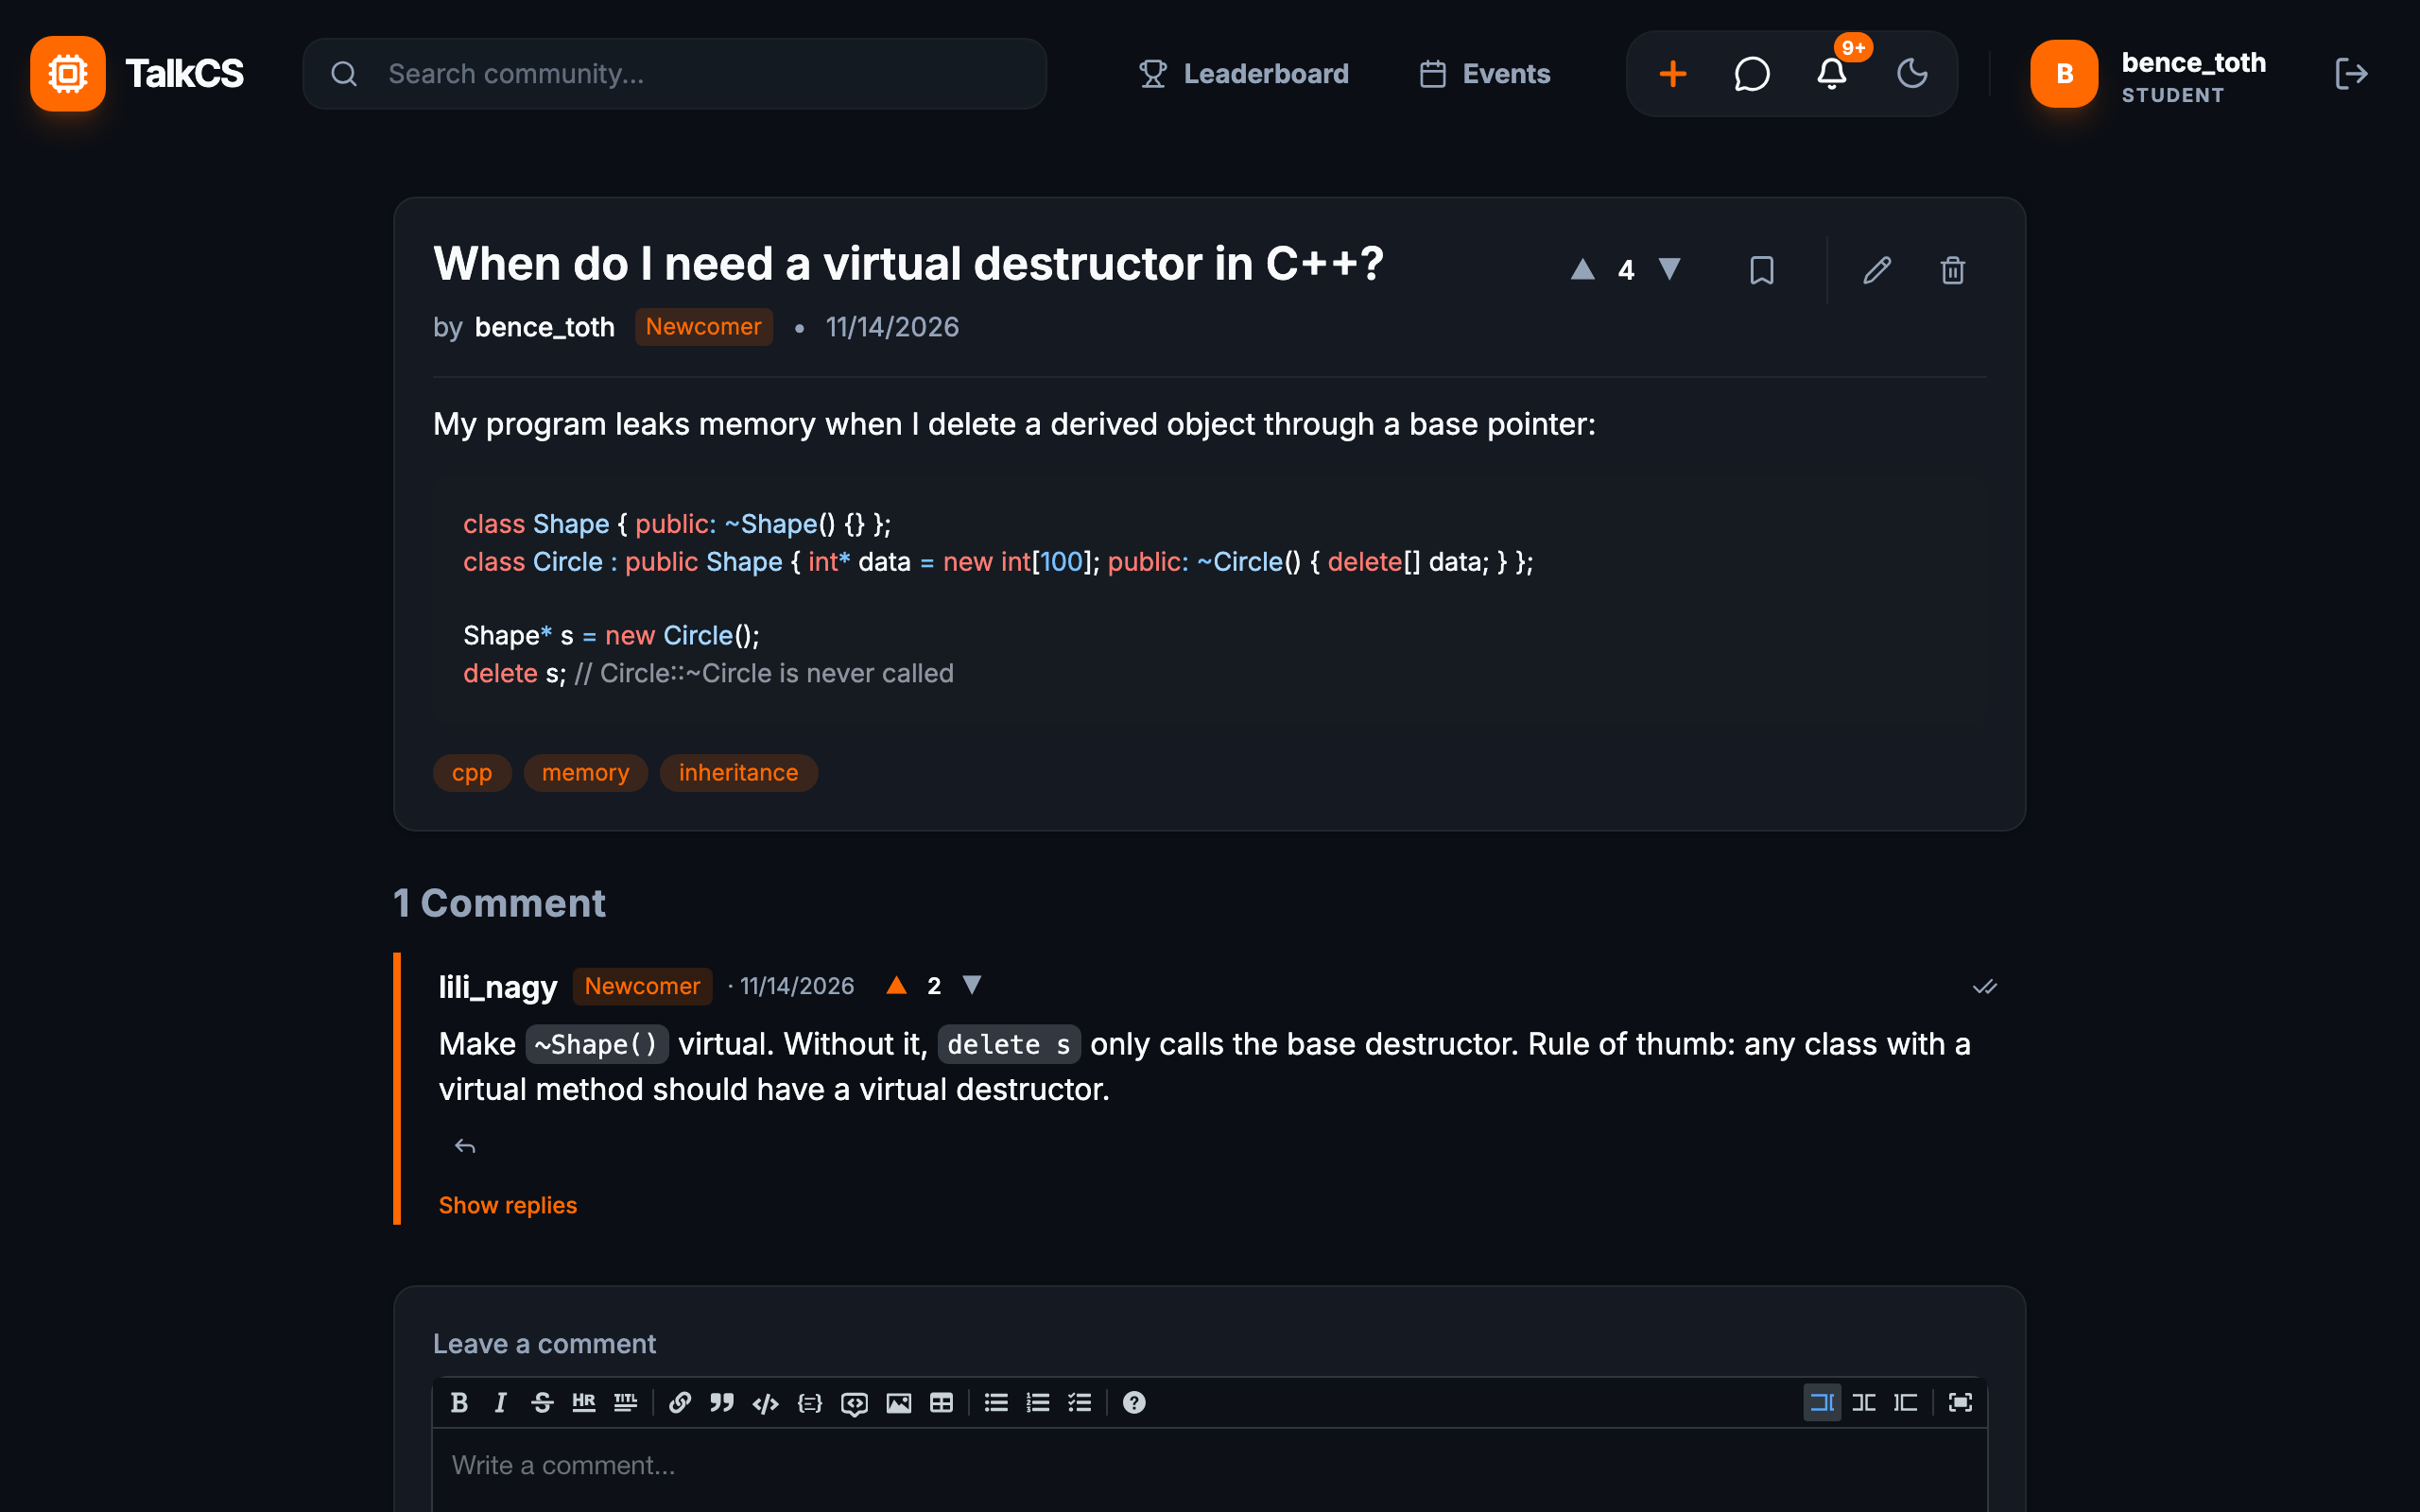
\includegraphics[width=\linewidth]{figures/screenshots/theme-dark.png}\caption{Dark mode}\end{subfigure}\\[1em]
    \begin{subfigure}{\textwidth}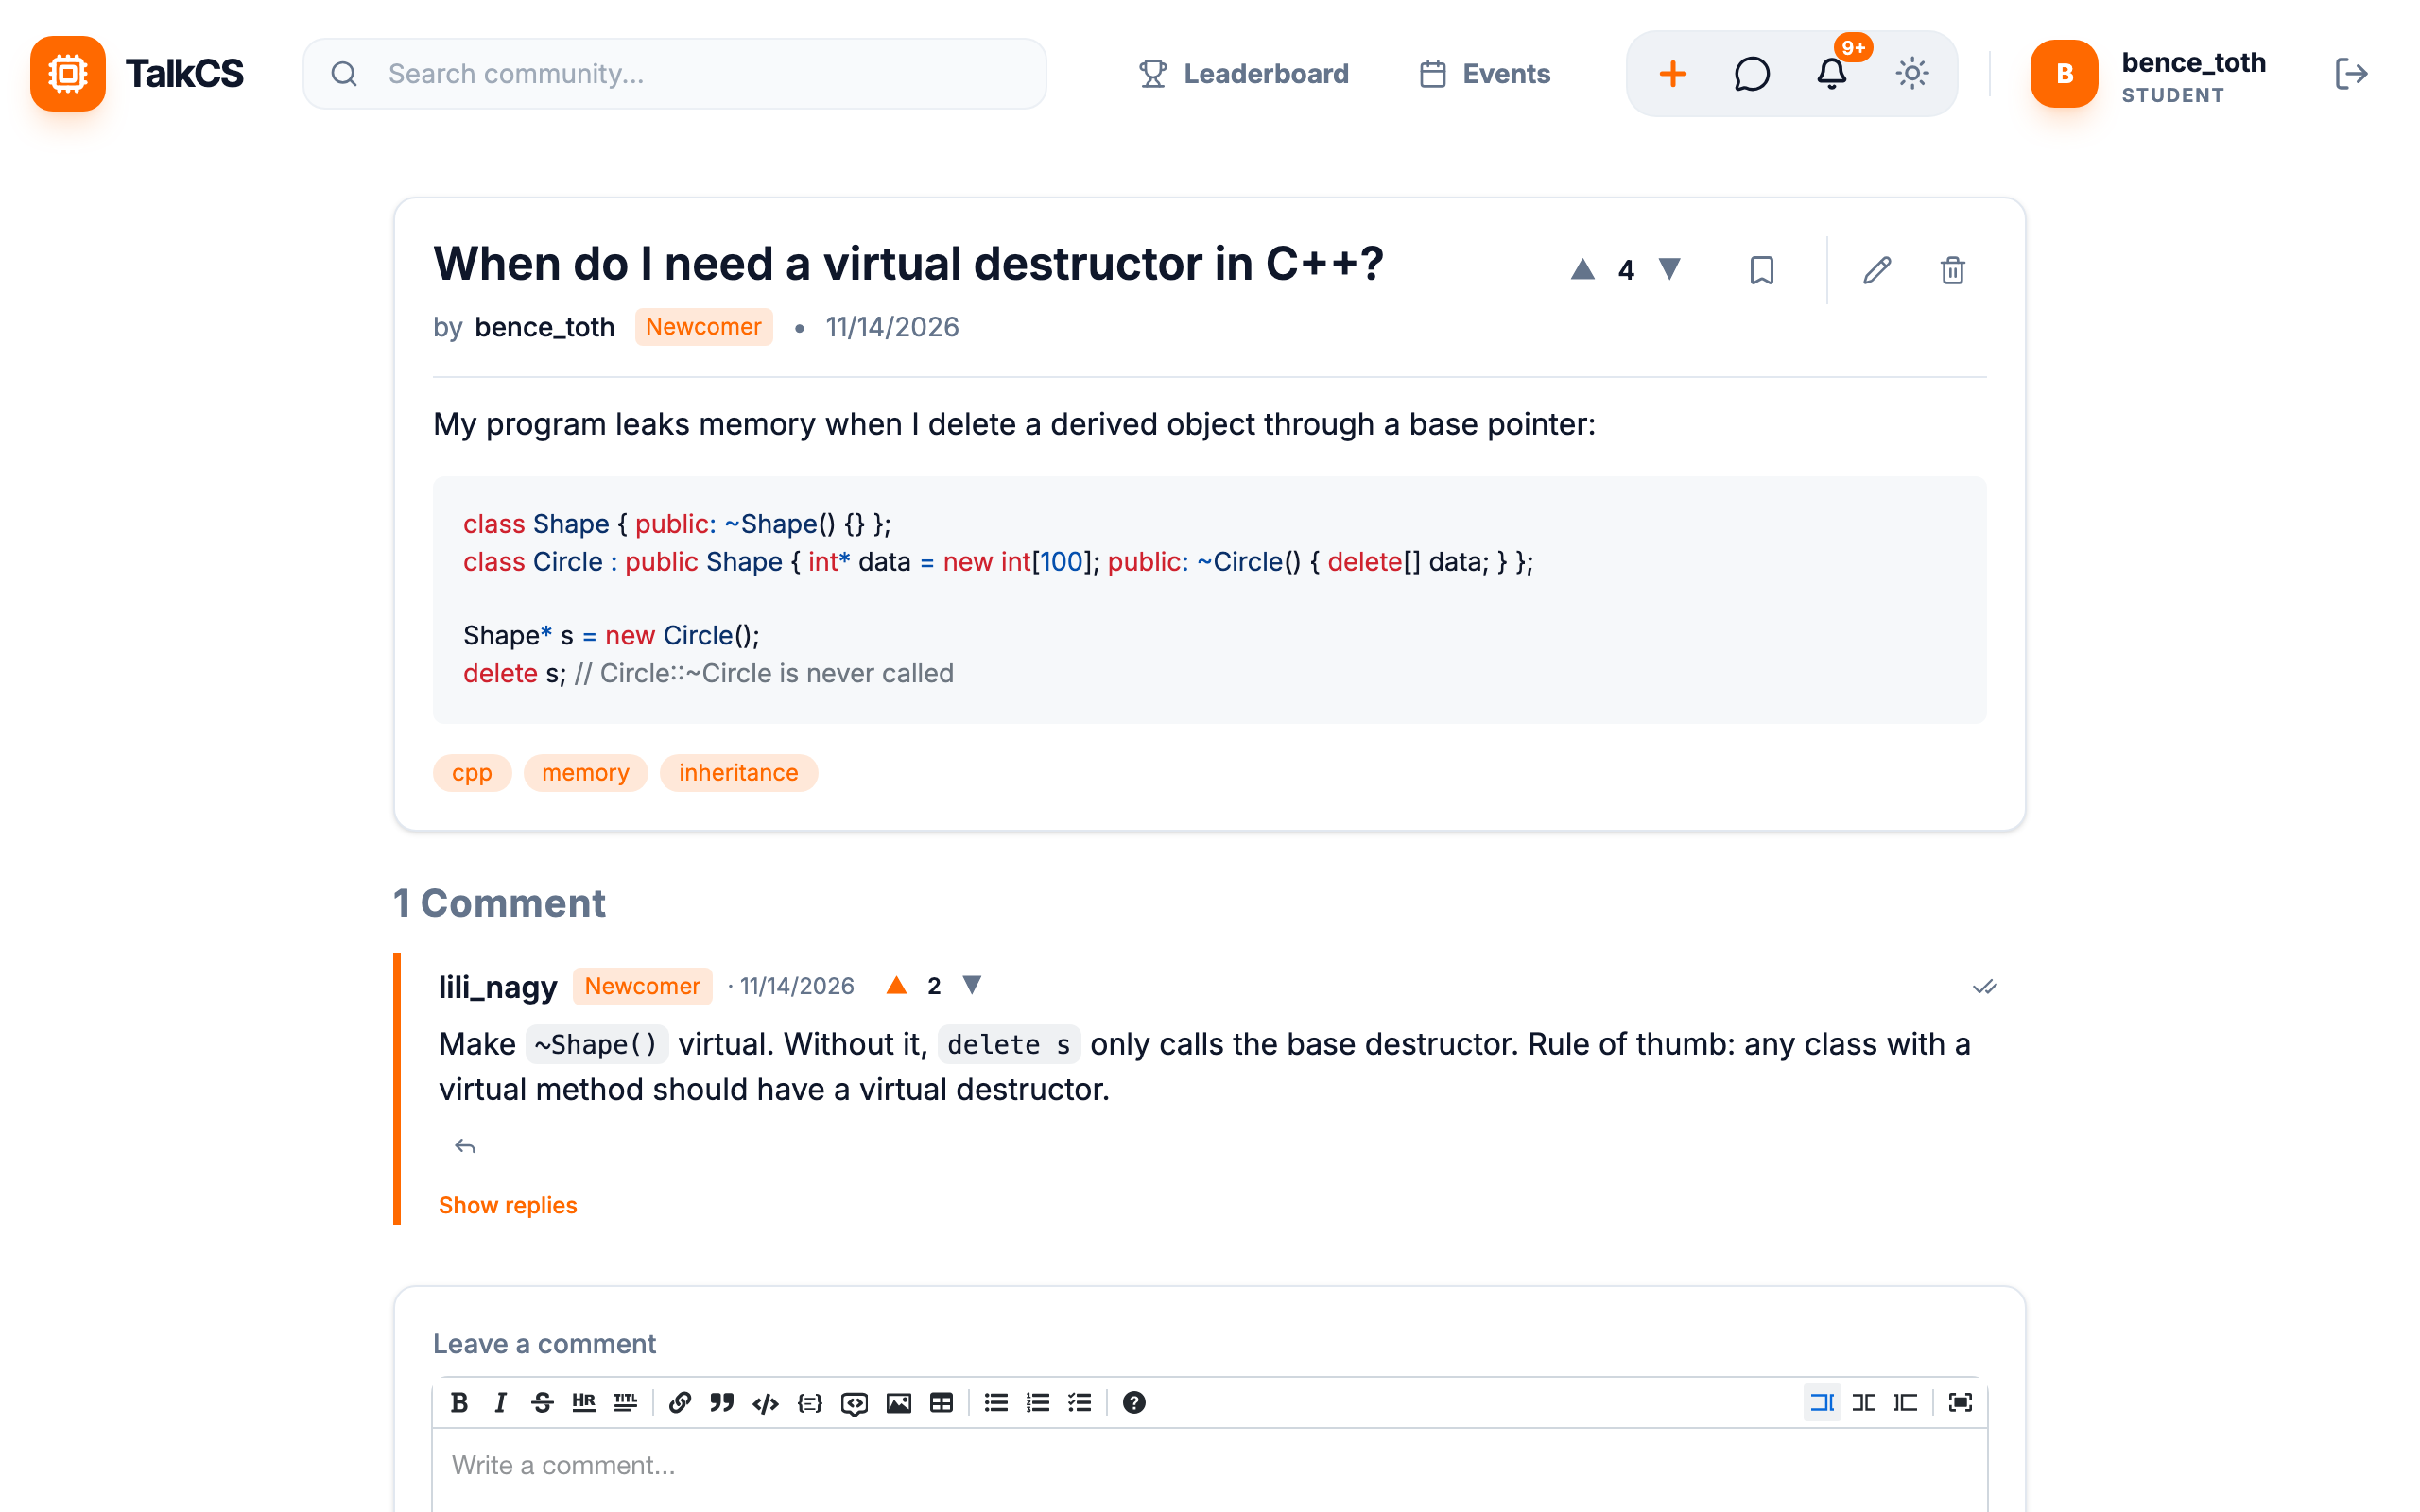
\includegraphics[width=\linewidth]{figures/screenshots/theme-light.png}\caption{Light mode}\end{subfigure}%
  }{%
    \fbox{\begin{minipage}[c][4cm][c]{\dimexpr\textwidth-2\fboxsep-2\fboxrule\relax}\centering\color{tcgray}\textbf{Screenshot placeholder}\\\texttt{theme-dark.png}\end{minipage}}\\[1em]
    \fbox{\begin{minipage}[c][4cm][c]{\dimexpr\textwidth-2\fboxsep-2\fboxrule\relax}\centering\color{tcgray}\textbf{Screenshot placeholder}\\\texttt{theme-light.png}\end{minipage}}%
  }
  \caption{TalkCS in dark and light mode}
  \label{fig:themes}
\end{figure}

% =====================================================================
\section{System Messages and Error Handling}

TalkCS provides contextual feedback to help users understand what happened and what
to do next. Short confirmations (for example \emph{``Post created successfully!''}) are
displayed as notifications in the top-right corner of the screen, and form errors are
shown next to the affected field. Table~\ref{tab:messages} lists the most common
messages, their cause, and the recommended action.

\begin{longtable}{@{}>{\raggedright\arraybackslash}p{0.30\textwidth} >{\raggedright\arraybackslash}p{0.33\textwidth} >{\raggedright\arraybackslash}p{0.30\textwidth}@{}}
  \toprule
  \textbf{Message} & \textbf{Cause} & \textbf{Recommended action} \\
  \midrule
  \endfirsthead
  \toprule
  \textbf{Message} & \textbf{Cause} & \textbf{Recommended action} \\
  \midrule
  \endhead
  \bottomrule
  \endfoot
  \bottomrule
  \caption{System messages and recommended user actions}
  \label{tab:messages}
  \endlastfoot
  Invalid email or password. & Incorrect login credentials were submitted. &
    Check the e-mail and password, or use the password recovery. \\
  Invalid email & The e-mail field does not contain a valid address. &
    Correct the address. \\
  Minimum 8 characters & The password chosen during registration is too short. &
    Choose a longer password. \\
  Email already exists & An account with this e-mail address already exists. &
    Log in, or recover the password of that account. \\
  Username already exists & The chosen username is taken. & Choose another username. \\
  Passwords do not match. & The two password fields on the reset page differ. &
    Type the same password into both fields. \\
  Invalid or expired reset link. Please request a new one. & The reset link is older
    than one hour or has already been used. & Request a new reset link. \\
  Cannot vote on your own post / comment / resource & The user tried to vote on their
    own content. & Voting is reserved for other users' content. \\
  Only post author can accept answers & Someone other than the question author tried to
    accept an answer. & Only the question author can do this. \\
  Category already exists & A category with this name exists. & Choose another name. \\
  Failed to create event. & The event could not be saved, e.g. because of a missing
    date. & Fill in all required fields and try again. \\
  Access Denied & The user has no permission for the action (e.g. a Student opening an
    administrator function). & Ask an administrator if the permission is needed. \\
  (redirect to the login page) & The session has expired after 24 hours or the token is
    invalid. & Log in again. \\
\end{longtable}
